%% Copyright 2019 Bernd Haberstumpf
%% License: CC BY-NC
\newsection{Humanoide Rassen}

Neben nat"urlich oder k"unstlich befruchteten Menschen hat es die Menschheit vor einem halben Jahrhundert geschafft, Menschen die sogenannten Mutanten aus artifiziell sequenziertem Erbmaterial zu klonen. Das Erbmaterial der Mutanten ist auf das Leben au\3erhalb der Erde hin optimiert. Mutanten werden in Zuchtbottichen der gro\3en Konzerne gez"uchtet. Sie werden in Ausbildungskadern ohne eigene Eltern gro\3gezogen und f"ur ihre jeweilige Aufgabe ausgebildet. Mutanten haben ein gr"auliche Haut und keine K"orperbeharung. Mutanten stehen im Dienst diverser Gro\3konzerne sowie des terranen Milit"ars in einem leibeigenen Verh"altnis, aus dem sie sich unter Umst"anden freikaufen k"onnen. W"ahrend Mutanten auf der Erde angefeindet werden, sind sie in den au\3erterrestrischen Kolonien ein nat"urlicher Teil der Gesellschaft.

\begin{figure*}[htbp]
      \centering
      \fbox{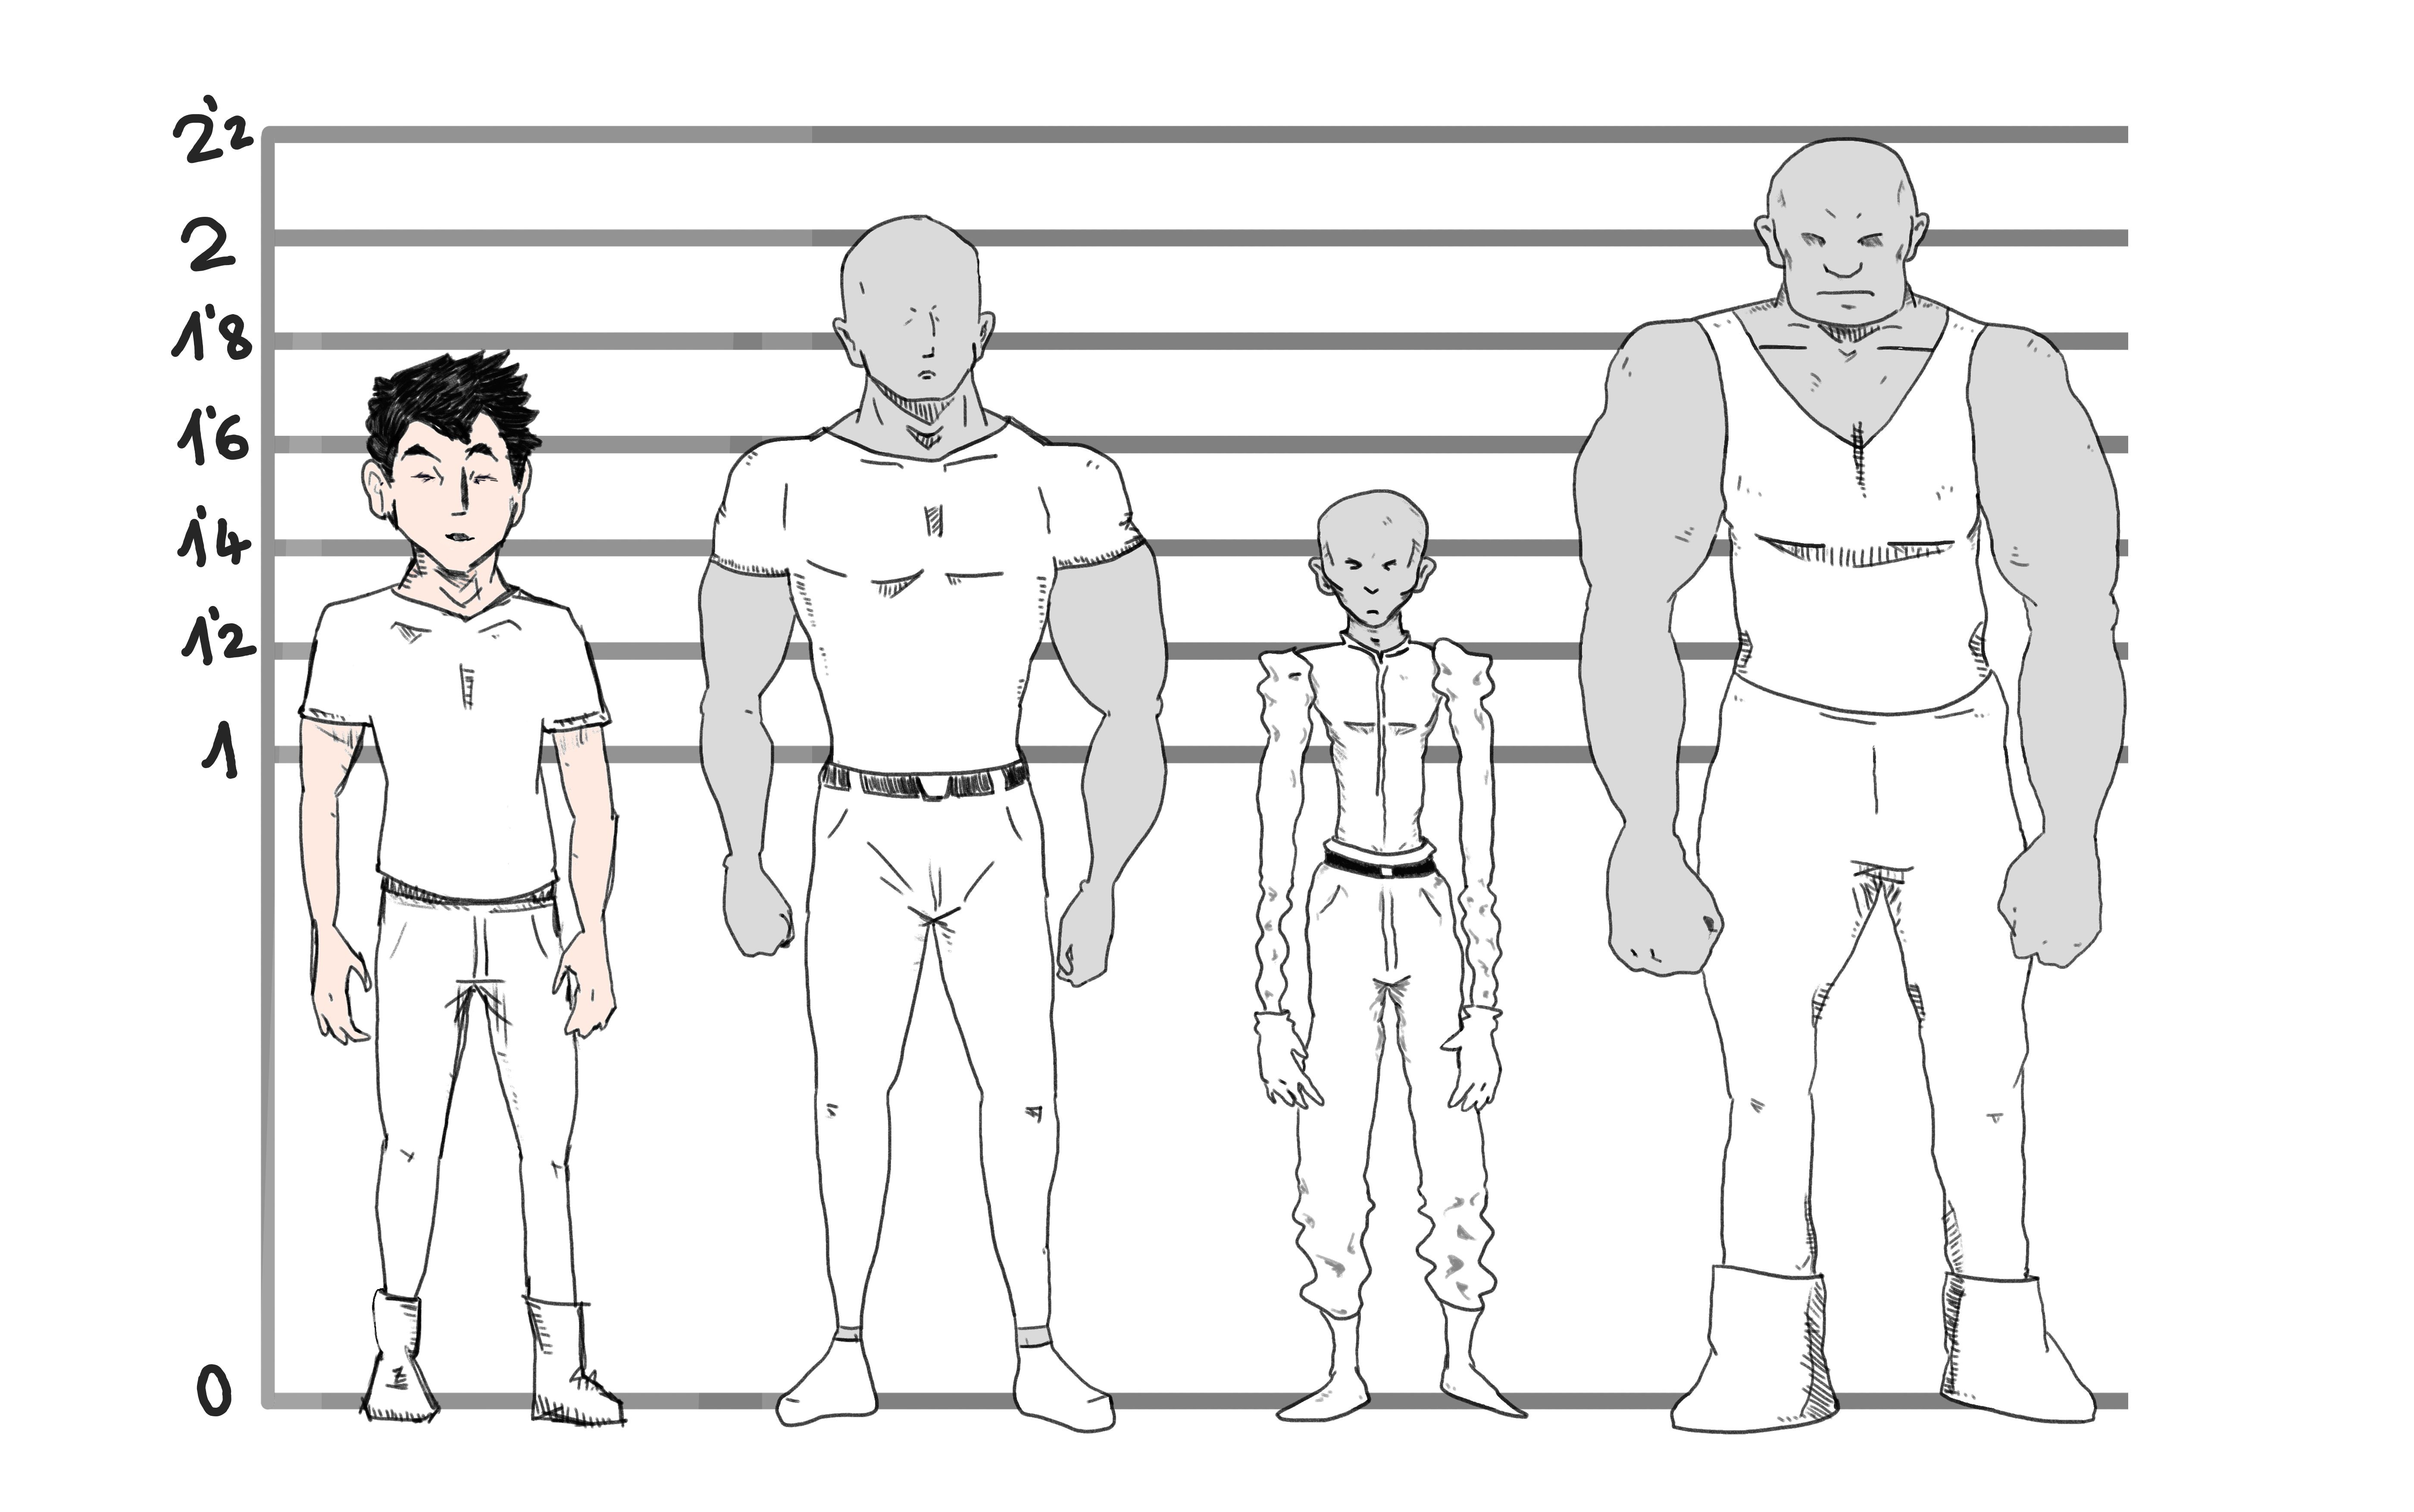
\includegraphics[width=0.75\textwidth]{images/races}}
      \newline{}Humanoide Rassen
      \label{fig:humanoide-rassen}
\end{figure*}
    

Im folgenden die relevanten Menschen und Mutantentypen.

\begin{description}
\item [Norms] Normal gebohrene Menschen werden Norms genannt. Seit der Besiedelung des Weltalls spielen die
      menschlichen Rassen keine so gro\3e Rolle mehr.
\item [Pure] Pure sind k"unstlich befruchtete, genetisch verbesserte Menschen. Das genetische Material wird vor der
      Befruchtung von negativen Genomen gereinigt. Pures sind Kinder der Superreichen und bilden einen signifikanten Teil der Oberschicht.
\item [Spacer] Spacer sind Humanoide, die ihr ganzes Leben in der Schwerelosigkeit verbracht haben. Bei Spacern haben
      sich Knochenmaterial und Muskel soweit zur"uck gebildet, dass sie sich nicht mehr ohne Exoskelett unter Schwerkraft wie auf der Erde oder dem Mars bewegen k"onnen. Stattdessen sind Spacer extrem geschickt in der Fortbewegung ohne Schwerkraft.
\item [Slags] Slags werden durch Strahlung mi\3gebildete Menschen genannt. Sie bilden den Bodensatz der
      humanen Gesellschaft.
\item [Alpha Mutant] Alphas sind die als Arbeiter in den extraterrestrischen Kolonien konzipierten Mutanten.
      Alphas sind deutlich kr"aftiger als Norms und haben einen deutlich stabileren und massigeren K"orperbau. Alphas haben eine gro\3e Resistenz gegen kosmische Strahlung und sind gut ger"ustet f"ur unterschiedliche Schwerkraftbedingungen. Alphas sind schwere Arbeit unter gef"ahrlichen Bedingungen gew"ohnt und haben meist einen gutm"utigen Charakter.
\item [Eta Mutant] Etas sind als Piloten und Personal f"ur Raumschiffe konzipiert. Sie sind nur 1,35 bis 1,50 Meter gro\3
      und drahtig. Optimiert f"ur Schwerkraftextreme und erh"ohte kosmische Strahlung sind sie f"ur den Einsatz auf Raumschiffen optimal angepasst.
\item [Omega Mutant] Omega Mutanten sind als Infanterist im Armeedienst gez"uchtet. Sie sind 1,90 bis 2,10 Meter gro\3.
      Omegas sind "ahlich wie Alphas extrem kr"aftig und haben eine nahezu unzerst"orbare Konstitution. Omegas sind von klein auf f"ur den Kampf ausgebildet, haben taktische Erfahrung und kennen den Umgang mit allen Waffensystemen.
\end{description}

\newsection{Technologie}

Ein Gro\3teil der Shadowrun-Regeln, Cyberware und die Matrix als Virtuelle Realit"at k"onnen "ubernommen werden.

Im folgenden ein kleiner Auszug von spezieller Technologie der 23.~Jahrhunderts.

\begin{description}
\item [ComLink] Ein ComLink wird zur drahtlosen Verbindung in das ComNetz genutzt. Das ComLink ist entweder als
      Mobilger"at mit AR Brille oder als Headware verf"ugbar.
\item [ComNetz] Ein ComNetz ist auf den meisten menschlichen Siedlungen etabliert. Das ComNetz ist eine virtuelle
      Computerwelt und Kommunikationsinfrastruktur. In das ComNetz bindet man sich per ComLink ein. Per Augmented Reality (AR) werden Informationen und Steuerelemente in das audiovisuelle Zentrum der Teilnehmer eingeblendet. Das ComNetz wird f"ur die Kommunikation, zur Informationsbeschaffung, f"ur Finanztransfers, zur Steuerung von Ger"aten etc.~genutzt. Um tiefer in das Netz einzutauchen und in einer vollsensorischen Virtuellen Realit"at einzutauchen, wird eine kabelgebundene Verbindung "uber eine Datenbuchse ben"otigt.
\item [Commandchip] Der Commandchip ist die Ankopplungszentrale an das Gehirn. Der Commandchip erlaubt es Augmented Reality (AR) Signale in     das Sehzentrum und das H"ohrzentrum einzuspielen wie auch alle anderen Headware anzubinden.
\item [Credcard] Eine Credcard ist das Pendant zum ehemaligen Papiergeld. Eine vorher mit Geld aufgeladene Karte kann an
      einen Zahlungsempf"anger gegeben werden oder es kann per ComLink Geld von einer Credcard transferiert werden.
\item [Datenbuchse] Eine Datenbuchse ist eine am Hinterkopf verbaute Kabelschnittstelle zu einer Headware.
\item [Fusionstriebwerk] Fusionstriebwerke bilden den Hauptantrieb von Raumschiffen. "Uber Man"ovrierd"usen werden
      Raumschiffe in die richtige Positionen gebracht, um die m"achtigen Fusionstriebwerke zur Beschleunigung oder zum Abbremsen zu benutzen. Fusionstriebwerke nutzen eine Kernfusion mit HE-3 als Brennstoff und Wasser als Treibmasse.
\item [Headware] Mit dem Gehirn verbundene Hardware im Kopf, z.B.~ein ComLink das das ComNetz direkt mit dem Gehirn
      verbindet.
\item [ID--Chip] Menschen und Mutanten werden durch einen im linken Arm unter der Haut implantierten ID--Chip
      identifiziert. Der ID--Chip dient als Pass oder auch der Autorisierung von Zahlungen. Mittels Near--Field-Communication kann ein Reader auf den ID--Chip zugreifen.
\item [Magnetstiefel] Mangnetische Stiefel dienen dazu, in Schwerelosigkeit auf einem Raumschiff oder einer Station zu
      laufen. Zur Aktivierung werden sie zusammengeschlagen.
\item[PAN] Ein PAN (Personal Area Network) ist ein technisches System im Kopf der Person und umf"asst z.B.~ einen Commandchip und   
      die Anbindungen des Girns an weitere Cyberware im K"orper wie auch angebundene Systeme au\3erhalb des K"orpers.
\item [Psychonauten] Psynchonauten sind Personen, die "uber eine kabelgebundene Verbindung das Gehirn
      einer anderen Person infiltrieren k"onnen. Dieser Gehirnscan erlaubt es, Gedanken, Erinnerungen und Gef"uhle des anderen zu erforschen. Da es sich um eine bidirektionale Verbindung handelt, erf"ahrt auch der Gescante evtl.~etwas "uber den Psychonauten. Ein Gehirnscan ist gef"ahrlich und kann zum Gehirntot der gescanten Person f"uhren.
\item [Raumanzug] Im 23.~Jahrhundert haben sich Raumanz"uge zu Tauchanz"ugen "ahnlichen Bodysuites entwickelt, die unter
      normaler Kleidung getragen werden k"onnen. Raumanz"uge sch"utzen vor Druck und Temperaturunterschieden. Zusammen mit Druckluftkanistern und Gesichtsmasken erlauben sie den Aufenthalt in Weltall.
\item [Riggersteuerung] Eine Riggersteuerug erlaubt es technische Ger"ate fern zu steuern. Die Riggersteuerung wird direkt im 
      Gehirn verbaut und mit dem Commandchip verbunden oder extern "uber die Datenbuchse angebunden.
\item[Talentchip] Talentsoft erweitert den Tr"ager "uber den Commandchip um neue geistige und physische F"ahigkeiten. 
\end{description}

\newsection{Waffen}

Im folgenden ein Auszug von im 23.~Jahrhundert gebr"auchlichen Waffen.
%% Wie die Waffen auf in Shadowrun gebr"auchliche Waffen abgebildet werden k"onnen ist jeweils angegeben.

%% TODO

\begin{description}
\item [Bolter] Ein Bolter ist eine semiautomatische elektrisch getriebene Faustfeuerwaffe.
\item [Gau\3kanone] Eine Gau\3kanone ist eine Waffensystem das auf Raumschiffen zum Einsatz kommt. "Uber mehrere Spulen
      werden Projektile in einem elektrisches Feld beschleunigt. Eine Gau\3kanone verschie\3t mit hoher Feuerrate Hochgeschwindigkeitprojektile und gilt als die durchschlagskr"aftigste Feuerwaffe im Sonnensystem.      
\item [Gefechtspanzer] Ein Gefechtspanzer ist ein Exoskelett mit starker Panzerung, eingebautem Raumanzug, Sensorik,
      Waffenplattformen und einem Jetpack. Ein Gefechtspanzer wird von Omega-Infanteristen eingesetzt.
\item [Multigun] Eine Multigun in den meisten F"allen eine sehr gro\3e Faustfeuerwaffe ist eine Railgun die es erlaubt zwischen     
      penetrierenden Projektilen und Schockmunition umzuschalten.            
\item [Plasmawerfer] Ein Plasmawerfer ist eine Infanteriewaffe, die von Omega-Mutanten in einem Kampfpanzer zusammen mit
      einem R"uckentornister getragen wird. Der Plasmawerfer verschie\3t hochenergetisches Plasma, das nahezu alles au\3er schweren Stahlplatten verbrennen kann.
\item [Railgun] Eine Railgun beschleunigt Hochgeschwindigkeitsprojektile entlang von zwei unter Strom gesetzten Stangen. Eine Railgun ist 
      Neben dem Bolter ist die Railgun die meistgenutzte Handfeuerwaffe. Die Railgun gibt es als Fautfeuerwaffe oder Gewehr zumeist in  vollautomatischer Ausf"uhrung. Railguns werden auch auf Schiffen als Verteidigung gegen anfliegende Geschosse genutzt.
\item [Raketenwerfer] Raketenwerfer sind eine der Hauptwaffensysteme von Raumschiffen.
\item [Vibrokling] Eine durch hochfrequente Vibration extrem scharfe Klinge.
\end{description}

\newsection{Institutionen}

\begin{description}
\item [Cynarian Corporation] Die Cynarian Corporation ist der zweitgr"o\3te Konzern im Sonnensystem mit Hauptsitz auf
      dem Mars. Cynairan wird durch ein Direktorium aus drei Personen geleitet. Durch eine geschickte Verhandlung gelang es Cynarian, HE-3 Sch"urfrechte auf dem Jupiter f"ur Cynarian und das Protektorat zu sichern.
      \item [Europ"aische F"orderation] Die Europ"aische F"orderation umfasst die ehemaligen Nationalstaaten Europas auf der Erde. Die Europ"aische F"orderation ist eine Quasi-Demokratie, regiert durch die technokratische Partei. Auf Druck der "Offentlichkeit hat die Europ"aische F"orderation Mutanten als illegale Einwanderer klassifiziert und interniert seitdem Mutanten. Ortsans"assige Konzerne wurden aufgefordert, Mutanten aus dem Dienst zu entlassen. Die Europ"aische F"orderation betreibt ein Raumflotte im erdnahen Orbit und zwei Orbitalfestungen, von denen eine zeitweise durch das Protektorat eingenommen wurde.
\item [Das Protektorat] Das Protektorat ist die Mutantennation, die sich nach dem Verbot von Mutanten in Europa
      auf der Erde etabliert hat. Das Protektorat wird auf der zivilen Seite durch den Protektor Avenger regiert, der sich als Widerstandf"uhrer etabliert hat. Auf milit"arischer Seite wird das Protektorat durch Lord Marshall Blackheart geleitet, die mit weiteren Omega-Kriegern der Streitkr"afte der Europ"aischen F"oderation zum Protektorat "ubergelaufen ist.
\item [Shigano-Kombinat] Das Shigano-Kombinat ist ein Konzern auf dem Mars, spezialisiert auf die Z"uchtung von
      Mutanten. Das Shigano-Kombinat bietet auch ein hochentwickeltes Spektrum an Cybertechnologie an. Das Shigano-Kombinat ist eine Abspaltung des Japanischen Kaiserreichs.
\item [Transnationaler Konzernrat] Der Transnationale Konzernrat ist der oberste Gerichtshof der transnationalen
      Konzerne. Er entscheidet in wirtschaftlichen und milit"arische Fragen, die die Konzerne betreffen.
\item [United Space Industries USI] Die USI ist der gr"o\3te Konzern im Sonnensystem mit Hauptsitzt auf Luna. Die USI
      besitzt eine Monopolstellung f"ur HE-3 Gewinnung im Saturnsystem und f"ur den Abbau von seltenen Erzen im Asteroideng"urtel. Die USI wird von dem Patriarchen McLean geleitet.
\item [Vereinte Nationen] Die Vereinten Nationen sind das oberstes Gremium der Nationalstaaten im Sonnensystem. Das
      Shigano Kombinat strebt eine Mitgliedschaft an. Das Protektorat ist kein Mitglied.
\end{description}

\newsection{Das jovianische System}

Als jovianisches System bezeichnet man den Jupiter und seine Trabanten. Das jovianische System beherbergt "uber 70  Himmelsk"orper. Im folgenden die wichtigsten f"ur den Plot.

\begin{description}
\item [Armageddon Raumkomplex] Der Raumkomplex ist eine Raumstation im Lagrange--Punkt L4 von Kallisto, ca.~1.9 Mio km         von Kallisto entfernt. Armageddon ist das Herz des Protektorats. Das aus stillgelegten Frachtern, Containern und
      Habitaten zusammengeschwei\3te und in Rotation versetzte Zylinderhabitat ist eine der gr"o\3ten Stationen im Sonnensystem. Armageddon beherbergt neben den Wohnvierteln des Protektorats auch eine Niederlassung der Cynarian Corporation sowie die Verwaltung des Protektorats. Der Name der Station stammt von einem Club, aus dem Fl"uchtlingslager in dem die Rebellion der Mutanten auf der Erde begann.
\item [Fenris] Die Fenris Raumstation ist der Hauptst"utzpunkt der Protektoratsflotte. Die Fenris Raumstation umkreist
      den Jupiter in einem etwas nierigeren Orbit als Kallisto. Zum Zeitpunkt der Ereignisse ist sie ca.~1.5 Mio km von Kallisto und ca 2.5 Mio km von Armageddon entfernt.
\item [Hellgate] Hellgate ist eine kleine Station auf dem nur wenige Kilometer durchmessenden jupiternahen Mond
      Adrastea in einem Orbit von 130'000 km (halbe Mond-Erde-Entfernung) innerhalb des Strahlungsg"urtels des Jupiter. Hellgate ist tief in den Eismantel des Mondes eingegraben und beherbergt die Cynarian HE-3-Raffinierie zur Erstveredelung des auf dem Jupiter gewonnen Rohgases. Der Mond beherbergt ebenfalls einen Milit"arst"utzpunkt des Protektorats.
\item [Jupiter] Der Jupiter ist der gr"o\3te Planet im Sonnensystem. Als der f"unfte Planet im Sonnensystem ist er der
      "au\3erste der inneren Planeten diesseits des Asteroideng"urtels. Jupiter ist 490 Mio km von der Sonne entfernt und hat einen Radius von 70'000 km. Er besitzt die doppelte Masse aller anderen Planeten im Sonnensystem und hat damit eine Gravitation von 2.5g. Jupiter ist ein Gasgigant ohne klare Oberfl"ache. Der Jupiter hat ein so starkes Gravitationsfeld, dass ein konstanter Partikelstrom aus geladenen Teilchen auf den Planeten einprasselt. Der Partikelstrom stellt eine letale Gef"ahrdung f"ur Mensch und Maschine dar. Der Jupiter besitzt wie der Saturn Ringe.
\item [Kallisto] Kallisto ist der "au\3erste der vier gro\3en Jupitermonde. 1.9 Mio km oder 6 Lichtsekunden vom Jupiter
      entfernt (5 fache Erd-Mond-Entfernung), bewegt er sich au\3erhalb des Strahlungsg"urtels. Kallisto ist der einzige Mond mit nennenswerten Siedlungen. Einige der Siedlungen wie die Hauptstadt Valhalla sind bereits vor dem Eintreffen des Protektorats entstanden und beherbergen ein buntes Konglomerat aus Gl"ucksrittern, Sekten auf der Suche nach Abgeschiedenheit, Verbrechersyndikaten und Piraten. Das Protektorat hat kein Mandat durch den Konzernrat f"ur Kallisto. Da sich jedoch "uber 500'000 Mutanten auf Kallisto angesiedelt haben betreibt das Protektorat eine kleine Garnison zur Bewahrung der "offentlichen Sicherheit beim Raumhafen in Valhalla. Valhalla ist tief in die Eisfl"ache des Mondes eingegraben. Valhalla umfasst mehrere zivile Stadtsektoren und einige Konzernsektoren. Valhalla wird offiziell durch mehrere Institutionen regiert, das Sagen im zivilen Teil der Stadt hat allerdings das Luna--Syndikat das sich im ehemaligen USI-Sektor Breidablik eingenistet hat und Luft und Wasseraufbereitung sowie das lokale Fusionskraftwerk beherrscht. Ein Flug zwischen Kallisto und dem Jupiter dauert in der Regel 10 Tage. % TODO Stadtviertel von Valhalla
\item [Nike] Nike ist die ehem.~Cynarian-Raumstation Neu--Gr"oningen. Neu--Gr"oning wurde nach Erlangen der
      Sch"urfrechte f"ur den Jupiter vom Mars zum Jupiter geschleppt und in den stabilien Orbit am Lagrange Punkt L5 von Kallisto gesetzt. Urspr"unglich als Forschungsstation konzipiert, beherbergt das Ringhabitat die lokale Verwaltung der Cynarian Corporation sowie mehrere High-Tech-Firmen und Forschungslabore von Cynarian und anderen Konzernen.
\end{description}

\newsection{Raumschiffe}

Folgende Klassen von milit"arischen Raumschiffen sind gebr"auchlich.

\begin{description}
\item [J"ager, Jagdbomber] J"ager und Jagdbomber sind Raumschiffe mit kurzer Reichweite und 1 bis 2 Mann Besatzung.
      J"ager und Jagdbomber sind f"ur den Raumkampf oder meist sogar f"ur den Atmosph"arenkampf ausgestattet. J"ager und Jagbomber sind mit Gau\3kanonen und Raketen bewaffnet. Bekannte Jagdbombertypen sind Lancer-Kanonenboote, Valkyrie  und Cobra Jagdbomber.
\item [Korvette] Eine Korvette ist ein mit einem starken Antrieb und leichter Bewaffnung ausgestattetes Kriegsschiff
      mit einer L"ange von etwa 50 Metern das auch interplanetar operieren kann. Ein Korvette hat "ublicherweise 5--10 Besatzungmitglieder und kann bis zu 10 Passagiere aufnehmen. Eine Korvette ist "ublicherweise mit Gau\3kanonen oder automatischen Railguns und Abwehrbewaffnung ausgestattet, gelegentlich auch mit Raketen. Korvetten haben oft einen Hangar f"ur ein Shuttle oder einen J"ager.
\item [Fregatten] Eine Fregatte ist der Korvette "ahnlich, ist aber mit einer L"ange von 100m deutlich gr"o\3er und besitzt
      neben einer "ahnlichen Bewaffung wie eine Korvette einen Hangar f"ur ca.~5 J"ager.
\item [Schlachtkreuzer] Ein Schachtkreuzer ist ein interplanetares Gro\3kampfschiff mit einer Gr"o\3e von 300 Metern,
      dass mit allen m"oglichen Waffensystemen ausgestattet ist, Platz f"ur Infanterieeinheiten und einen Hangar f"ur J"ager bietet.
\item [Flottentr"ager] Ein Flottentr"ager ist ein bis zu 500 Metern gro\3es Kampfschiff zur Aufnahme von
      Jäger Steffeln und Infanterieeinheiten in Kompaniest"arke.
\end{description}

Folgende Raumschiffe spielen f"ur die Geschichte potentiell eine Rolle.

\begin{description}
\item [Flottentr"ager Donar] Einer der beiden Flottentr"ager des Protektorats und Flaggschiff des Protektorats unter
       dem Kommando von Lord Commander Steeler.
\item [Flottentr"ager Martell] Der zweite Flottentr"ager des Protektorats unter dem Kommando der Eta Espina.
\item [HeM03-Mine] HE-3 Mine auf den Jupiter. Wurde durch einen Unfall zerst"ort.
\item [HeM05-Mine] HE-3 Mine auf dem Jupiter. Konnte nach einem Attentat gerettet werden.
\item [Kreuzer Hyperion] Leichter Kreuzer von Cynarian.
\item [Fregatte Isamu] Die Fregatte Isamu ist das Schiff mit dem die Delegation des Shigano--Kombinats zusammen mit den 
      Vertretern der Europ"aischen F"oderation der im jovianischen System eingetroffen ist.
\item [Kreuzer Pendragon] Die Pendragon ist der Kreuzer des Protektorats.
\end{description}

\newsection{Bekannte Personen}

\begin{description}
\item [Colonel Scholz] Sicherheitschef der Cynarian Corporation im jovianischen System.
\item [Dr.~Petrova] Technische Leiterin der HE-3 Minen f"ur die Cynarian Corporation auf dem Jupiter.
\item [Director Eric Vandemool] Leiter der Cynarian Unternehmungen im Jovianischen System. Anw"arter auf einen
      Vorstandsposten.
\item [Espina] Eta Mutant. Kommandantin der Martell.
\item [Commander Lockhead] Omega Mutant. Kommandat der Garnison auf Kallisto Valhalla.
\item [Hato] Omega Krieger und Leibw"achter von Protector Avenger. Ehemaliger Angeh"origer des Shigano Kombinats.
\item [Kriegsmeister Jos\'{e} \frqq{}Toro\flqq{} Alvarez] Norm. Ausbilder der Jagdverb"ande des Protektorats.
\item [Lord Commander Grendel] Omega Mutant. Komandant auf der Fenris Station.
\item [Lord Commander Steeler] Omega Mutant. Kommandant der Donar.
\item [Lord Marshall Blackheart] Omega Cyborg. Oberbefehlshaberin der Protektoratsstreitkr"afte.
\item [Nemessis] Slag Cyborg. Duke des Luna Syndikats auf Kallisto und Herr "uber Valhalla.
\item [Protector Avenger] F"uhrer des Protektorats.
\item [Rhino] Alpha Mutant. Administrator von Armageddon.
\item [Sarana] Gesandte des Kombinatsrates.
\item [Seraph] Eta Mutant. Flugleiter des J"agerverbandes auf der Hellgate Station.
\item [Staatssekret"ar Luc Duval] Abgesandter der Europ"aischen F"orderation.
\item [Thunderbolt] Omega Mutant. Adjutant von Blackheart.
\end{description}